\en

The Linux kernel is a Free/Libre/Open-Source project providing value to
billions of people daily, representing 96.3\% of the top one million web
servers and 85\% of smartphones worldwide. The magnitude that the project has
reached over the years makes the addition of features, as well as handling bugs
and security vulnerabilities, potentially affect a significant number of
people, demonstrating the importance of maintaining the kernel
\citep{linuxdata}.

Maintaining the Linux kernel is a complex task, as the project contains more
than 19 million lines of code and has had over thirteen thousand contributors
throughout its lifespan \citep{linuxquantity}. Given the magnitude of the Linux
kernel project, it is unrealistic to expect that all contributors have
consistently followed the best programming practices and principles in every
contribution made to the project. Consequently, it is expected that a
significant amount of low-quality code artifacts will be found in the source
code, which could hinder or compromise the maintenance of the project and the
addition of new features.

As stated by \citet{driverdef}, device drivers are a ``piece of software whose
aim is to control and manage a particular hardware device, hence the name
device driver.'' Device drivers are a major part of the Linux kernel,
representing 66\% of the source code, and are responsible for managing
essential elements such as keyboards, mice, and GPUs \citep{marcelo}. When the
kernel opts to support new hardware, it necessitates alterations to existing
device drivers or the creation of new ones, making maintaining device drivers a
critical duty of the Linux community.

The AMD Display driver in the Linux kernel is responsible for enabling AMD GPUs
to operate correctly in desktop Linux environments, which is an essential task,
given that AMD GPUs represented 19\% of the personal GPU market in 2023
\citep{gpumarket}. When we interacted with the maintainers of the AMD Display
driver, they shared with us their challenges regarding one of the
characteristics of low-quality code artifacts: duplicated code, which hampers
the maintenance of the driver.

In searching for solutions to the AMD Display driver problem related to
duplicated code artifacts, we found tools capable of determining, given two
code artifacts, whether they are duplications of each other. However, the
formal literature on code duplication mainly focuses on optimizing the accuracy
of these tools for this specific task. These solutions do not address our
problem, as we cannot provide a complete codebase and have the tools return the
code duplications within it. Moreover, they do not guide us on how to mitigate
the code duplications after detection, necessitating the exploration of
alternative solutions.

Given the unsuccessful results of our search in the formal literature, we
turned to gray literature for solutions but were also met with limited success.
The best solutions we found in the gray literature were primitive, merely
identifying every pair of code files that are duplications. The code files in
the AMD Display driver containing duplicated code typically have specific code
unique to each file. Therefore, a solution that identifies duplication in a
deeper context is necessary to find accurate duplications within the Linux
kernel context. 
The list of gray literature tools examined in this exploratory research 
is available in Appendix A \ref{app:gray}.

\section**{Research Design}

\label{sec:intresearch}

Our studies and observations reveal that the code duplication problem described
in the previous section cannot be fully addressed by existing tools in
either the formal or gray literature. To fill this gap, we propose an approach
to identify and mitigate code duplications specifically within the Linux
kernel. Our approach includes the development of a tool capable of detecting
duplicated functions within the kernel and establishing strategies for
addressing these duplications.

\begin{figure}[h]
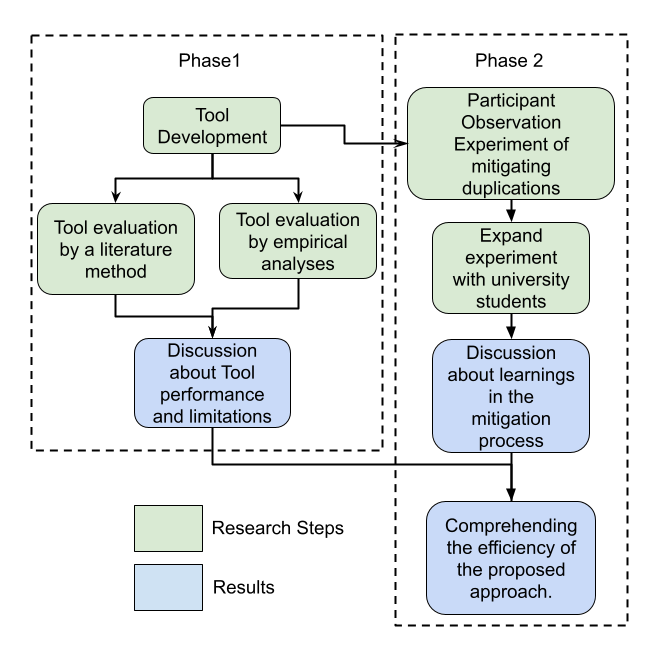
\includegraphics[scale=0.7]{research_design}
\caption{Diagram of the research design.}
\label{fig:reDesign}
\end{figure}

This research aims to identify patterns of software engineering techniques, such as refactoring methods commonly used to address code duplications. These patterns will serve as a guide for future contributors in mitigating code duplication issues within this context. To investigate our approach, we are developing a tool to identify duplicate code in the Linux kernel, explicitly targeting parts of the AMD Display driver code. We are then refactoring portions of this code and submitting patches to maintainers, providing evidence of the tool's accuracy in detecting duplicate functions. Our research design follows a multi-method approach, structured into two phases, each employing different research methods.

In \textbf{Phase I}, we propose, develop, and validate a tool capable of
identifying code duplications at the function level within C codebases. We
expect this tool to effectively detect code duplications in the Linux kernel,
as preliminary investigations suggest that kernel code files often contain a
mix of duplicated and unique functions. To validate the tool, we will use a
triangulation method, comparing its results with established code duplication
databases referenced in the literature, and conducting an empirical analysis on
a randomly selected set of files from the AMD Display driver, which our tool
flags as containing duplications. A detailed explanation of our validation
process is provided in Chapter \ref{cha:method}.


Upon completing the first phase, we anticipate having a validated tool for
identifying code duplications within the Linux kernel context. We will then
proceed to the second phase, which focuses on strategies for mitigating these
duplications. In \textbf{Phase II}, our objective is to identify practical
approaches to address the code duplications detected in the Linux kernel. To
achieve this, we have designed an ethnographic approach that enables us to
interact with the Linux development community and gather artifacts that either
support or challenge our proposed mitigation strategies. Figure
\ref{fig:reDesign} summarizes the research steps proposed in this study.


\section**{Manuscript Structure}


This manuscript consists of five more chapters. Chapter \ref{cha:back} presents
the literature overview for code duplication detection (main definitions,
current approaches in the literature), a brief description of the Linux kernel,
and a review of refactoring methods used throughout this research. Chapter
\ref{cha:tool} presents our proposed tool to detect code duplication in the
Linux kernel, describing all the main components.  Chapter \ref{cha:method}
describes the research methods selected to guide our work. Chapter
\ref{cha:results} shows the first results obtained from the research methods to evaluate
our proposed tool and presents the current research stage and the work plan,
with the addition of a discussion about our preliminary results.
